\chapter{Quaternionisches Apfelm"annchen}
\rhead{Quaternionisches Apfelm"annchen}
\begin{refsection}
\chapterauthor{Tabea M\'endez, Christian Schmid}
\lstdefinestyle{Matlab}{
  numbers=left,
  belowcaptionskip=1\baselineskip,
  breaklines=true,
  frame=L,
  xleftmargin=\parindent,
  language=Matlab,
  showstringspaces=false,
  basicstyle=\footnotesize\ttfamily,
  keywordstyle=\bfseries\color{green!40!black},
  commentstyle=\itshape\color{purple!40!black},
  identifierstyle=\color{blue},
  stringstyle=\color{orange},
  numberstyle=\ttfamily\tiny
}
\lstdefinestyle{OpenCL}{
  belowcaptionskip=1\baselineskip,
  breaklines=true,
  xleftmargin=\parindent,
  language=C,
  showstringspaces=false,
  basicstyle=\footnotesize\ttfamily,
  keywordstyle=\bfseries\color{green!40!black},
  commentstyle=\itshape\color{purple!40!black},
  identifierstyle=\color{blue},
  stringstyle=\color{orange},
  numberstyle=\ttfamily\tiny
}

\section{Mandelbrot-Menge}

\subsection{Einf"uhrung}
Die Mandelbrot-Menge (Abbildung \ref{fig. appleman}), auch bekannt als
''Apfelm"annchen'', umfasst eine Menge von Punkten der komplexen Ebene,
die gemeinsam eine fraktale Struktur bilden\footnote{Ein geometrisches
oder mathematisches Gebilde mit einer fraktalen Struktur, ist ein
Gebilde,  dessen (selbst"ahnliche) Form innerhalb des Gebildes immer
wieder in kleineren Formen vorkommt. \cite{fraktal}}. Sie wurde nach
dem franz"osischen Mathematiker Beno\^it Mandelbrot benannt, der die
Mandelbrot-Menge im Zusammenhang mit einer Studie der nahe verwandten
Julia-Mengen, im Jahre 1980 entdeckte. \cite{wiki}\\[-0.95cm]
\begin{figure}[ht!]\centering
\begin{adjustbox}{scale=0.45, keepaspectratio}
	\begin{tikzpicture}[>=latex, scale=1]
	\def\re0{7.5-0.6*15/2.6};
	\def\im0{0};
	\node at (0,0) {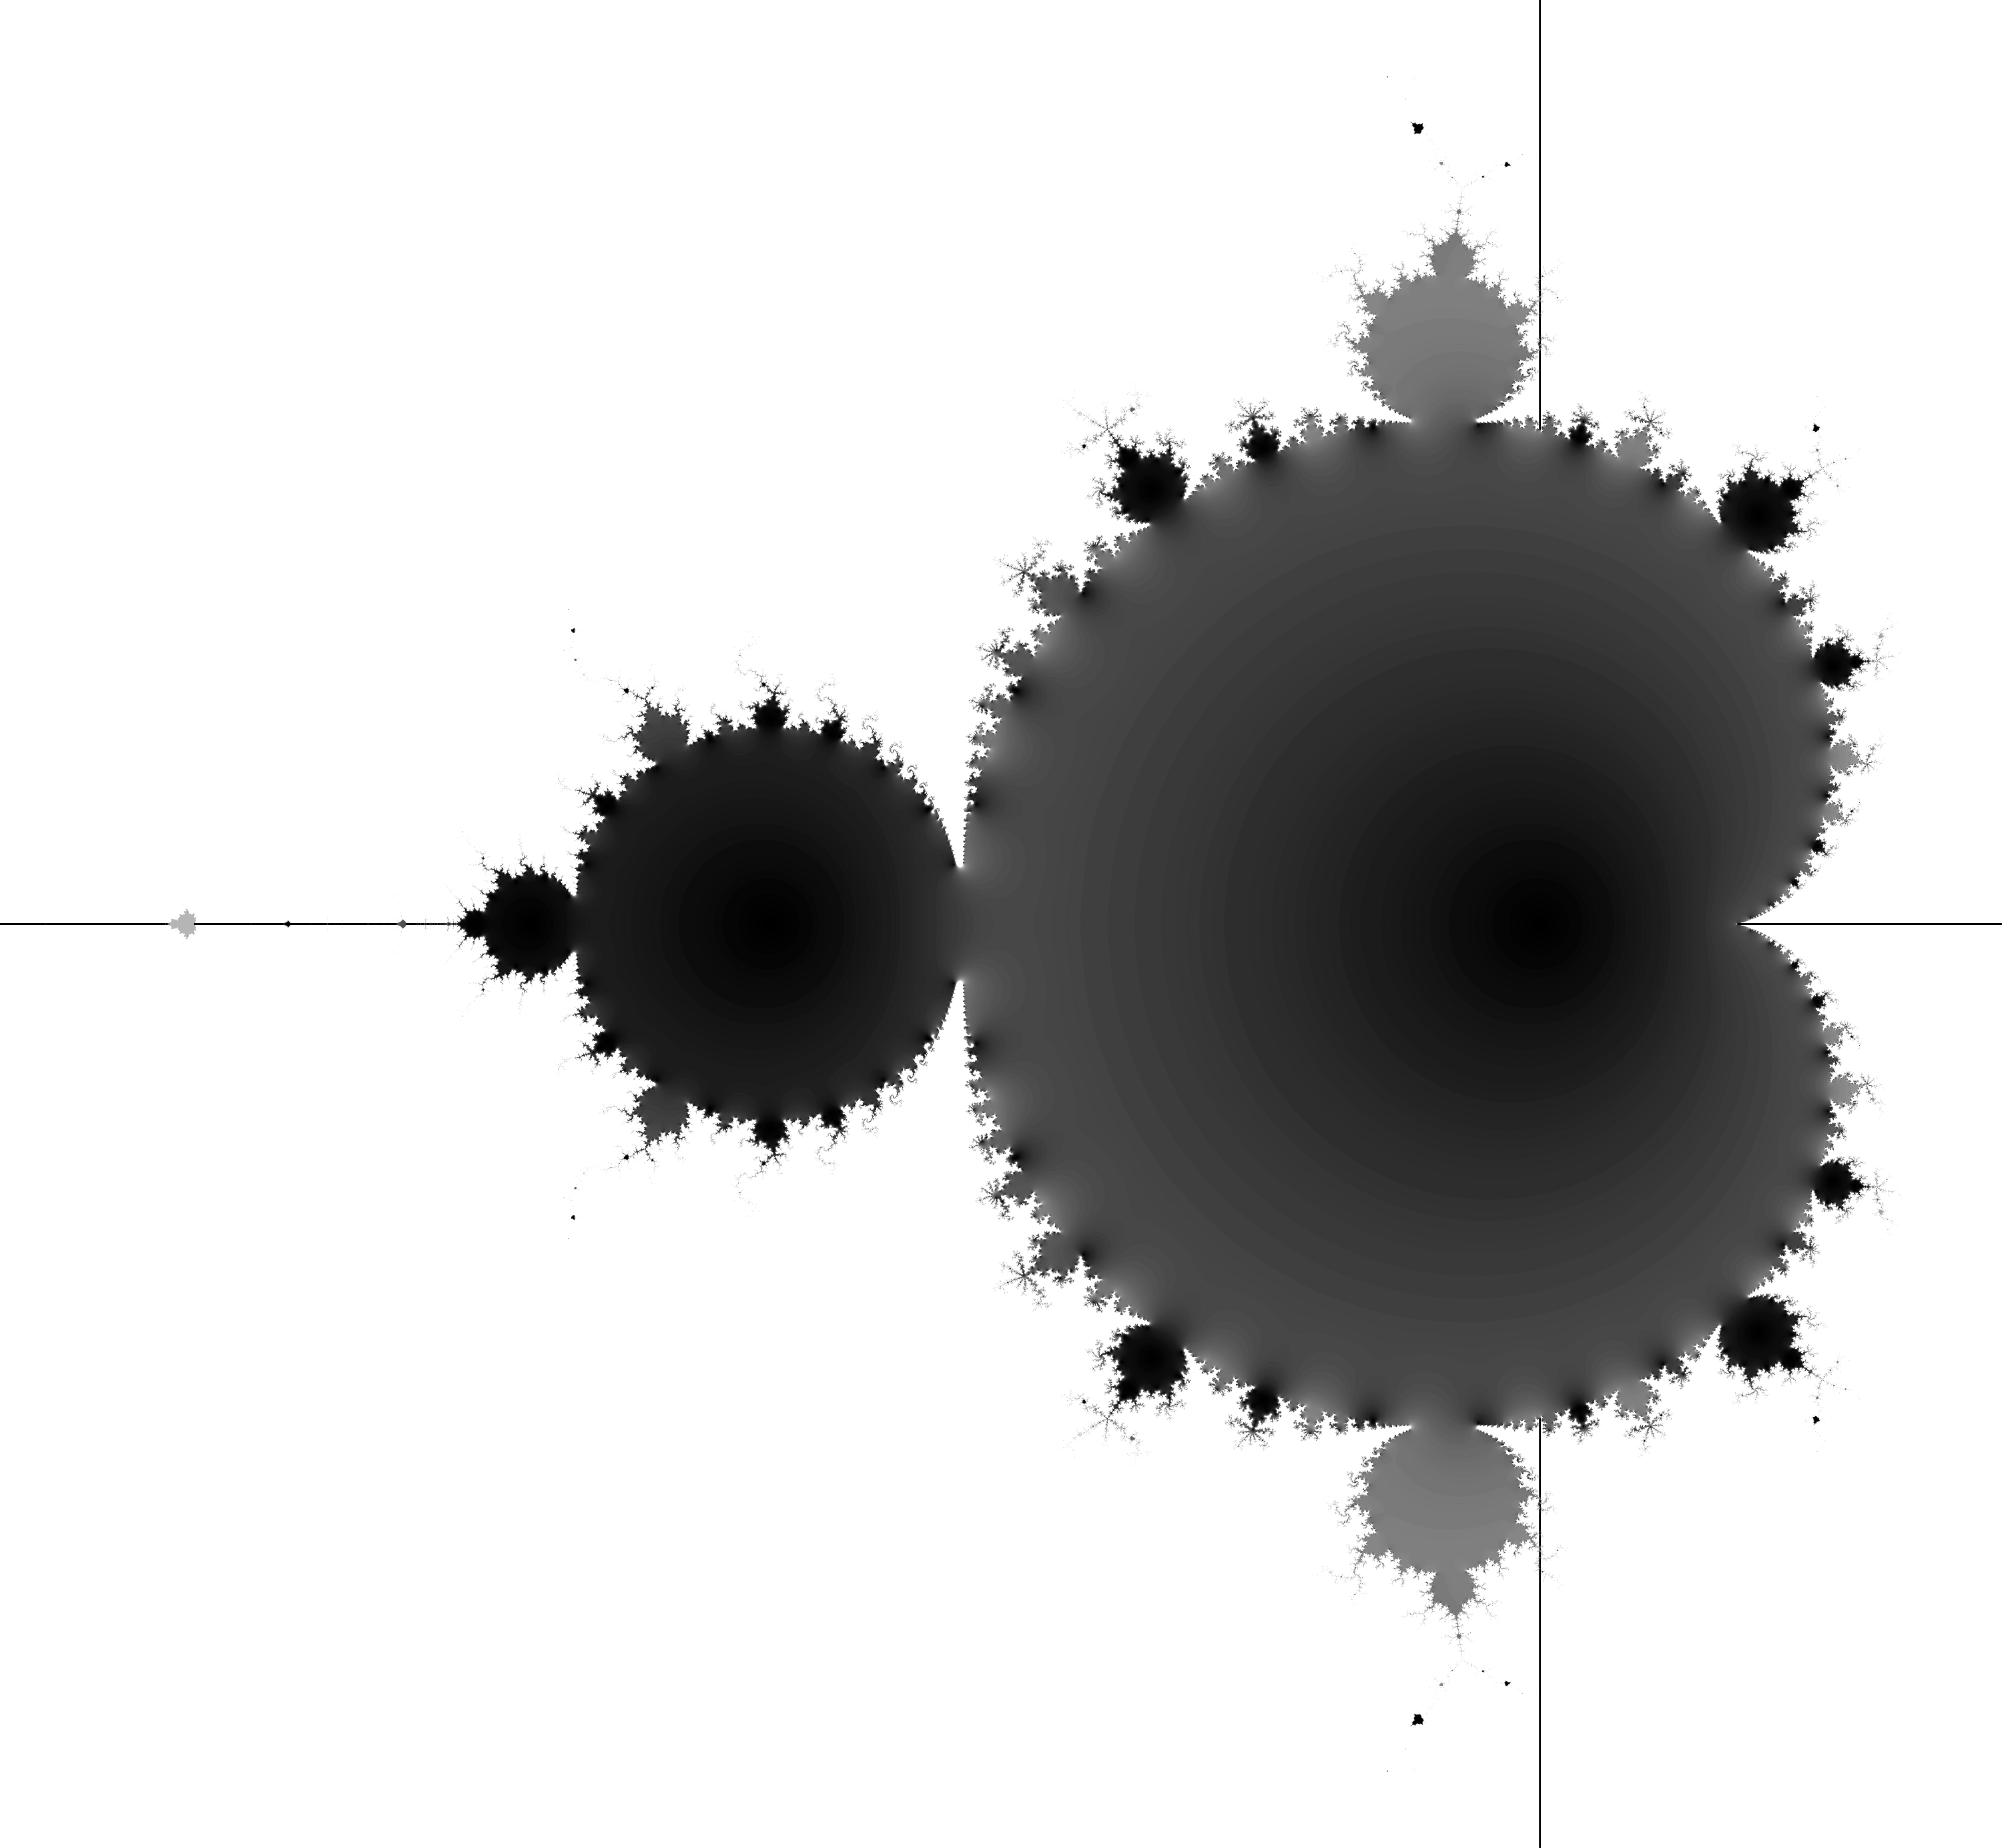
\includegraphics[width=15cm]{apfel/pic/apfelroman0251200koordinatenkomp.png}};
	\draw[->,line width=2](\re0+0.6*15/2.6-0.1,\im0)--++(0.15,0)node[below]{\large Re};
	\draw[->,line width=2](\re0,\im0+1.2*15/2.6-0.1)--++(0,0.15)node[right]{\large Im};

\end{tikzpicture}

\end{adjustbox}
% 			\includegraphics[width=0.58\textwidth]{pic/3048_MK_appleman.png}
\caption{Mandelbrot-Menge (Apfelm"annchen)}
\label{fig. appleman}
\end{figure}

\subsection{Definition}
Um die Mandelbrot-Menge $\mathbb{M}$ zu finden, wird f"ur jede komplexe
Zahl $c\in\mathbb{C}$ die Iteration der quadratischen Funktion
\begin{equation}
	f_c(z) = z^2+c
	\label{equ. itformel}
\end{equation}
untersucht. Anschliessend wird der Parameter $c\in\mathbb{C}$ danach
klassifiziert, ob die Iteration
\begin{equation}
	z_{n} = z_{n-1}^2+c\quad\text{ f"ur }\quad n\rightarrow\infty \quad\text{ mit }\quad z_0 = 0
	\label{equ. rekformel}
\end{equation}
divergiert oder beschr"ankt bleibt. Bleibt sie beschr"ankt, so geh"ort
$c$ zur Mandelbrot-Menge. Die Mandelbrot-Menge kann also folgendermassen
definiert werden:
\begin{equation}
	\mathbb{M} = \{c\in\mathbb{C}\;|\; f_c^i(0) \text{ bleibt beschr"ankt}\}
	\label{equ. defMandelbrotmengeComplex}
\end{equation}	


\subsection{Eigenschaften}
Die $c$'s der verschiedenen Teilgebiete der Mandelbrot-Menge
weisen jeweils ein charakteristisches Verhalten auf. So lassen sich
grunds"atzlich vier Verhaltensweisen unterscheiden.
\begin{itemize}
\item $f_c^i(0)$ (Formel \ref{equ. itformel}) strebt gegen einen
bestimmten Wert (Konvergenz).
\item $f_c^i(0)$ konvergiert gegen einen Grenzzyklus, der Periodenl"ange
zwei oder mehr. Beispielsweise $c=-1$ konvergiert gegen den Grenzzyklus
(-$1$, $0$, -$1$, \dots) mit Periodenl"ange zwei.
\item $f_c^i(0)$ wiederholt sich nie, aber bleibt beschr"ankt.
\item $f_c^i(0)$ strebt gegen unendlich (Divergenz).
\end{itemize}
In Abbildung \ref{fig. grenzzyklen} sind die Teilgebiete der Grenzzyklen
mit den jeweiligen Periodenl"angen dargestellt. Der ''K"orper'' der
Mandelbrot-Menge hat die Periodenl"ange eins und stellt somit das Gebiet
der Konvergenz dar. \cite{wiki} \\[-0.8cm]
\begin{figure}[ht!]\centering
	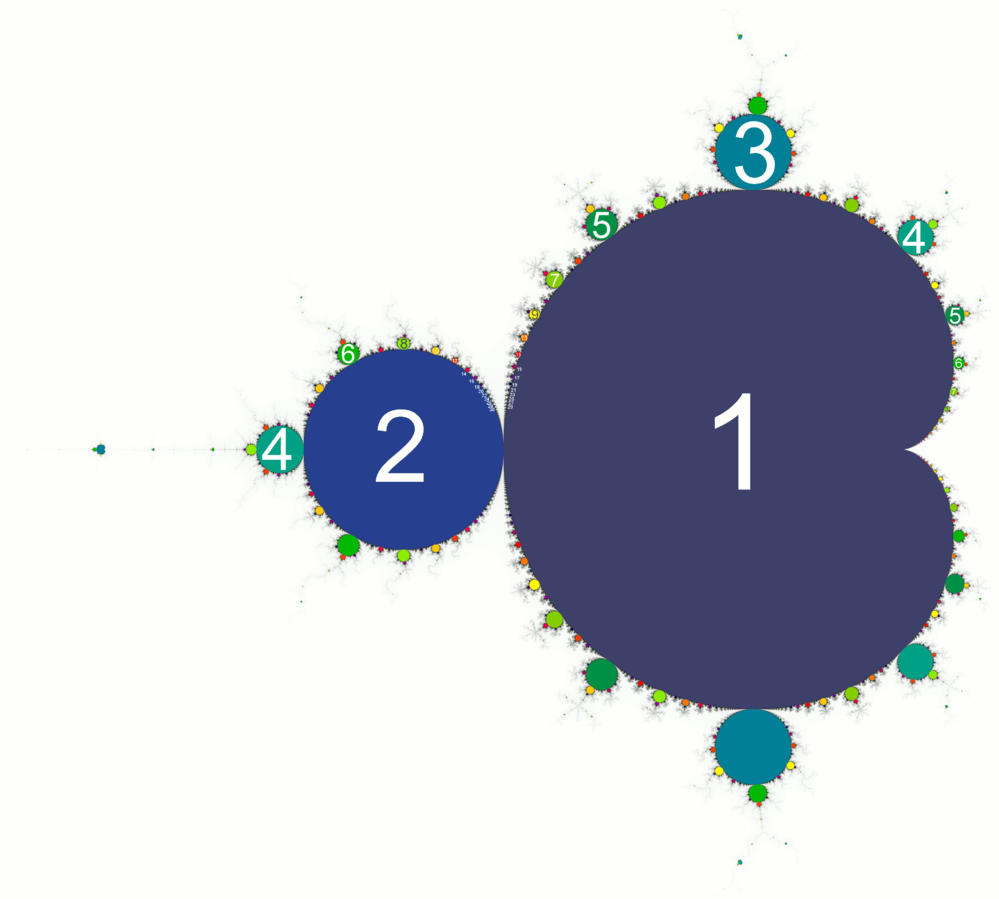
\includegraphics[width=0.5\textwidth]{apfel/pic/perioden_mandelbrotmenge.png}
	\caption{Teilgebiete mit den verschiedenen Periodenl"angen (1-7) der Grenzzyklen \cite{wikiBild}}
	\label{fig. grenzzyklen}
\end{figure}

\subsection{Bezug zur Julia-Menge}
Die Mandelbrot-Menge ist nahe verwandt mit der Julia-Menge. Der
Unterschied zu dieser liegt darin, dass bei der Julia-Menge $c$ konstant
bleibt und der Anfangswert $z_0$ variiert. Die Julia-Menge zu dieser
konstanten Zahl $c$ ist dann der Rand der Menge aller Anfangswerte $z_0$,
f"ur die $f_c^i(z_0)$ beschr"ankt bleibt.

Es kann gezeigt werden, dass die Mandelbrot-Menge auch "uber die
Julia-Mengen bestimmt werden kann. Dies, da sich die Mandelbrot-Menge
aus allen $c$'s zusammensetzt, f"ur die die zugeh"orige Julia-Menge
zusammenh"angend ist. In Abbildung \ref{fig. julia_mandelbrot}
sind zu einigen Werten $c$ jeweils die dazugeh"orende Julia-Menge
abgebildet \cite{wiki}.

\begin{figure}[ht!]\centering
	\begin{adjustbox}{scale=0.5, keepaspectratio}
		\begin{tikzpicture}[>=latex, scale=1]
	\definecolor{blueT}		{RGB}{0,0,220};
	\def\re0{7.5-0.6*15/2.6};
	\def\im0{0};

	\node at (7.8,4.8) {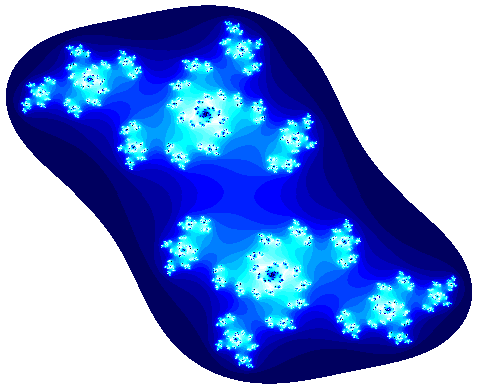
\includegraphics[width=5.5cm]{apfel/pic/julia005j072.png}};
	\node at (7.8,-4.8) {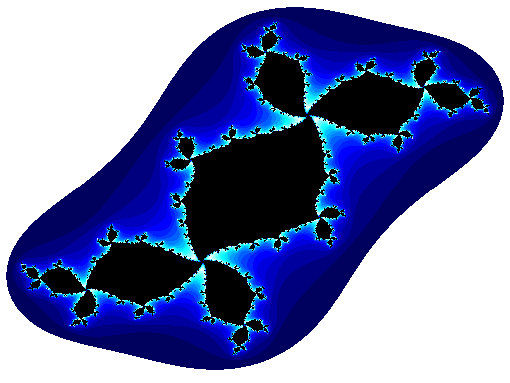
\includegraphics[width=5.5cm]{apfel/pic/julia-015j-075.png}};
	\node at (-2.8,4.2) {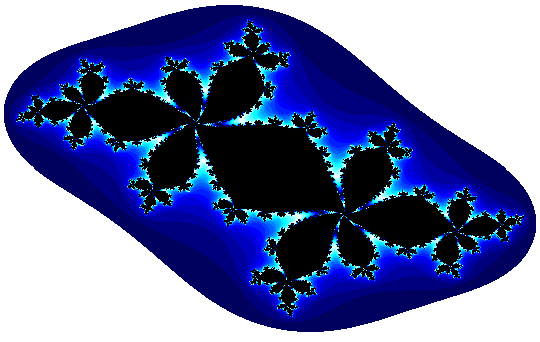
\includegraphics[width=5.5cm]{apfel/pic/julia-05j055.png}};
	\node at (-3.2,-4.2) {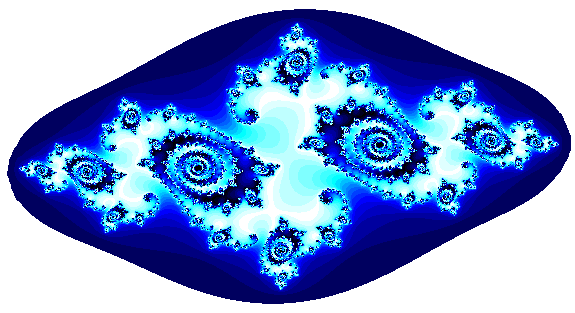
\includegraphics[width=7cm]{apfel/pic/julia-075j-015.png}};

	\node at (0,0) {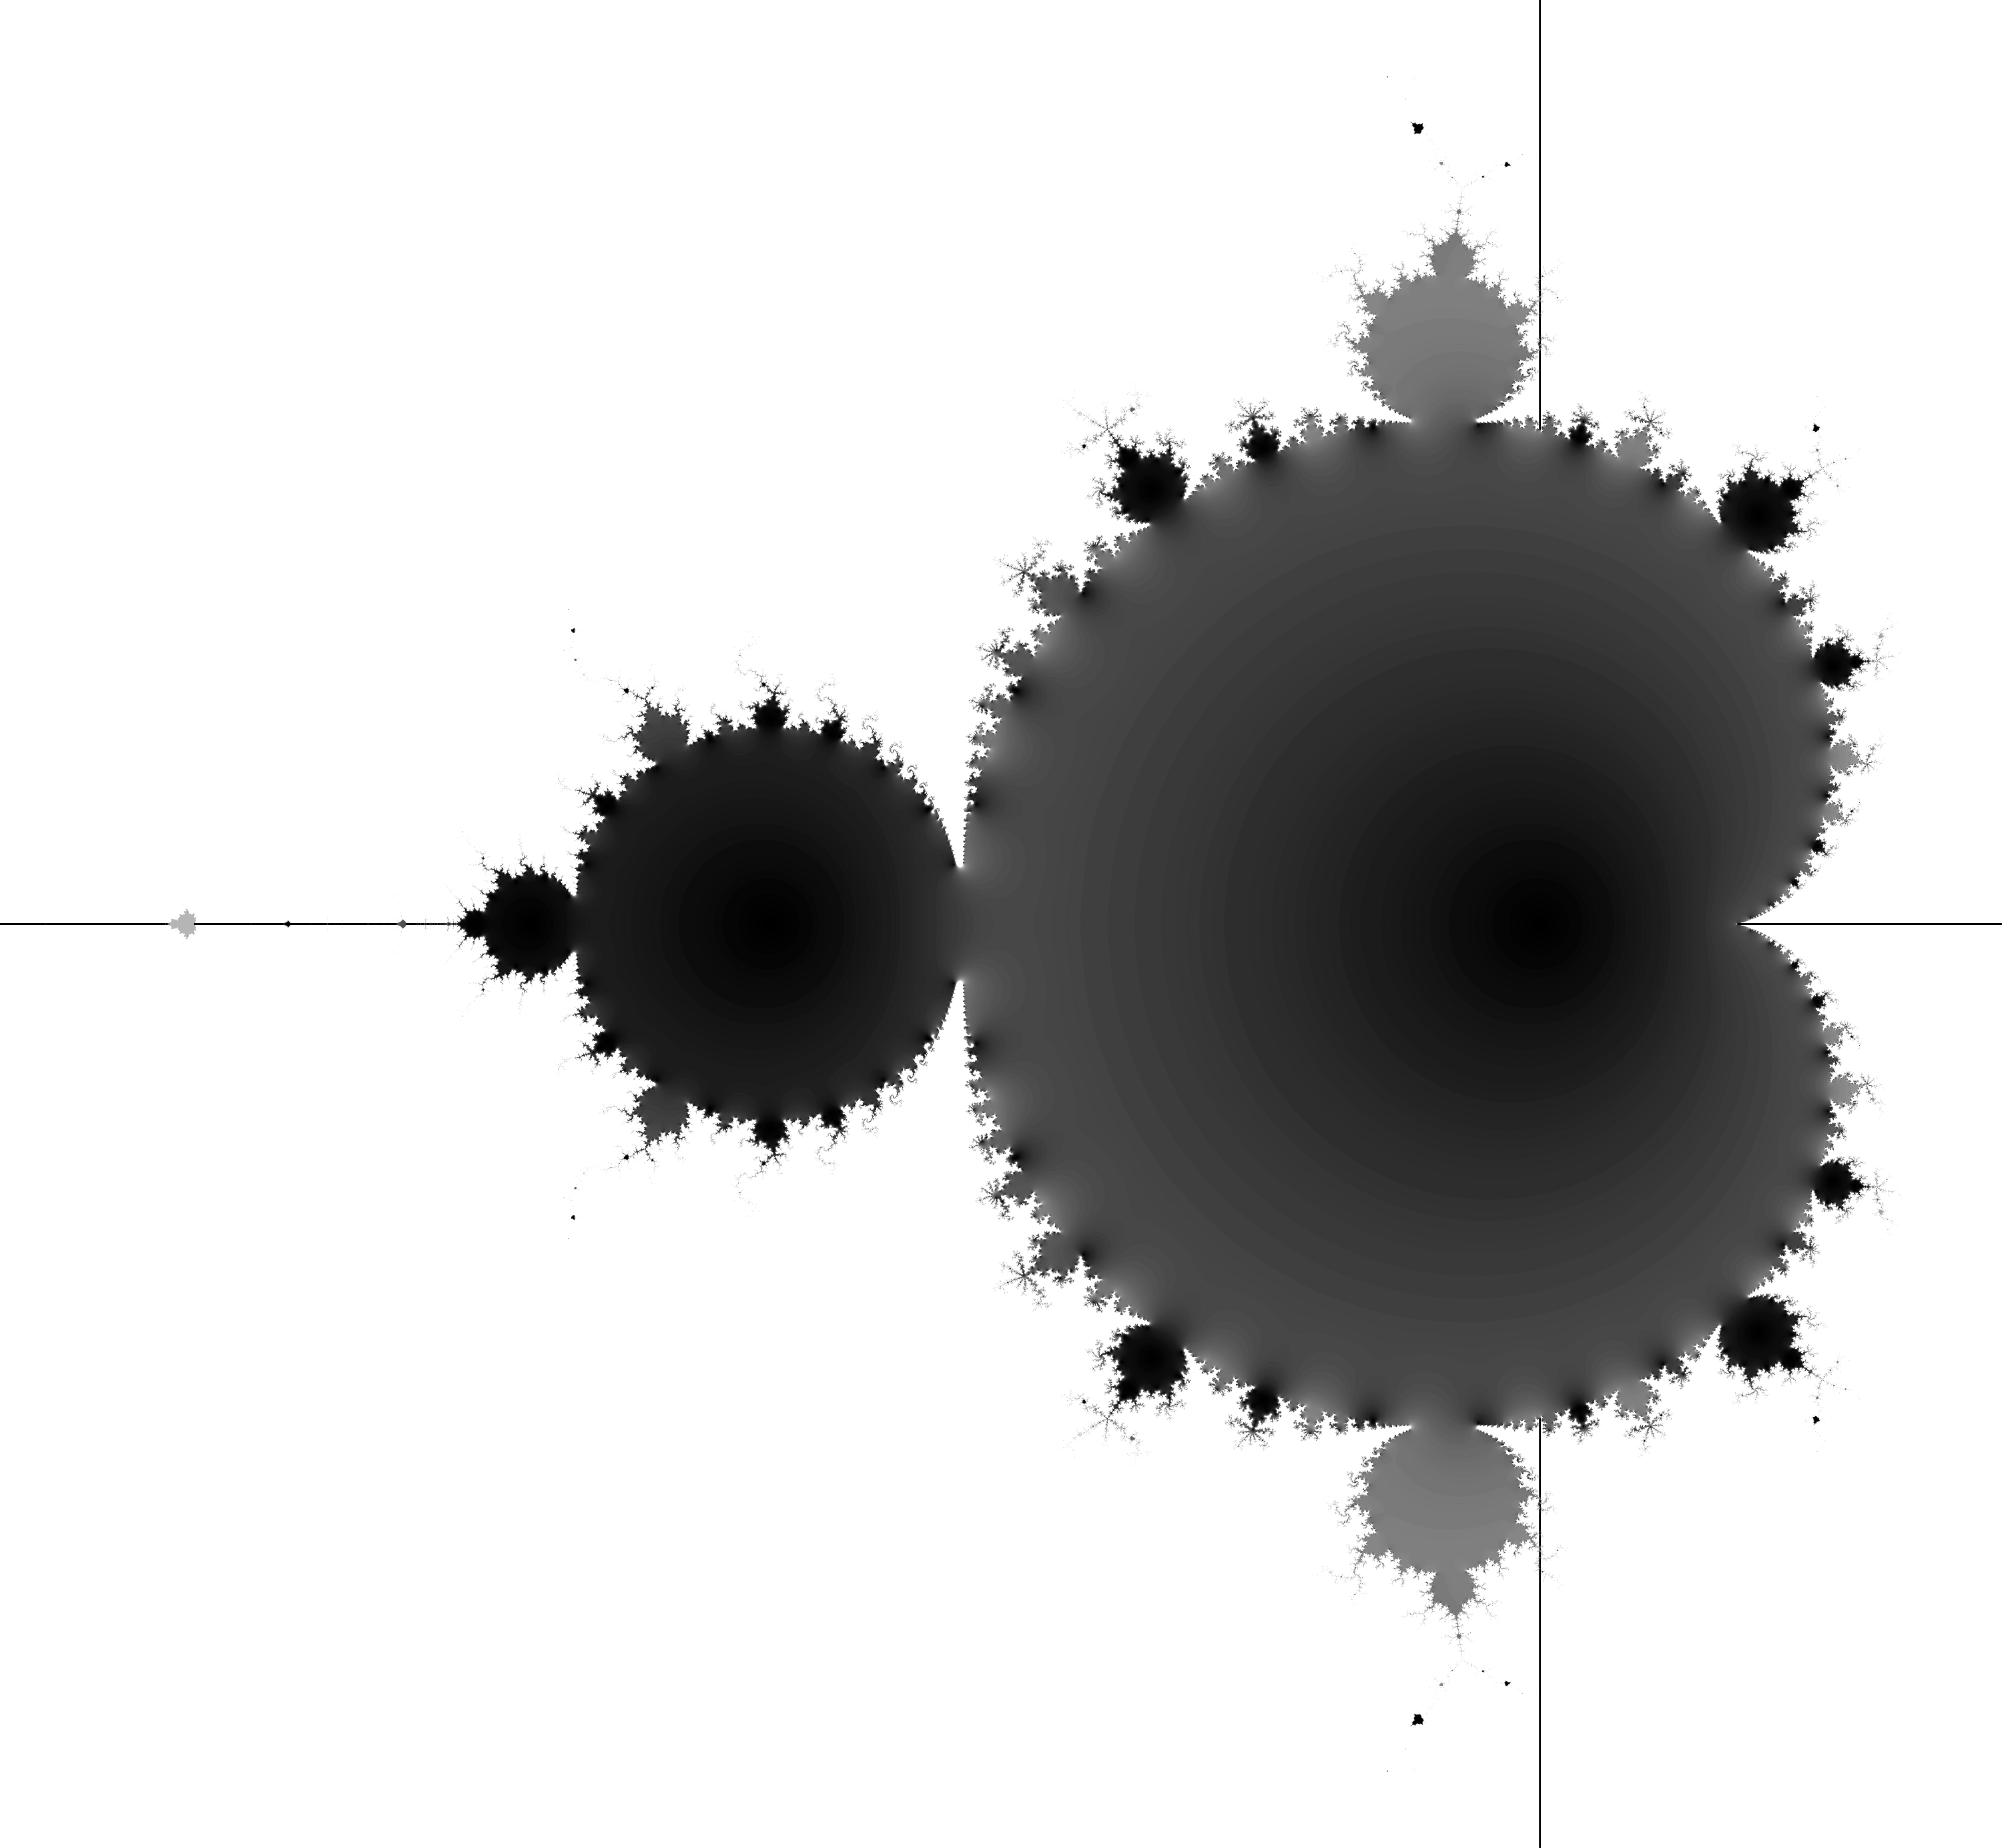
\includegraphics[width=15cm]{apfel/pic/apfelroman0251200koordinatenkomp.png}};
	\draw[->,line width=2](\re0+0.6*15/2.6-0.1,\im0)--++(0.15,0)node[below]{\large Re};
	\draw[->,line width=2](\re0,\im0+1.2*15/2.6-0.1)--++(0,0.15)node[right]{\large Im};


	\draw[blueT, fill] (\re0+0.05*15/2.6,\im0+0.72*15/2.6) circle (4pt);
	\draw[blueT, line width=1.5] (\re0+0.05*15/2.6,\im0+0.72*15/2.6) ++(0.2,0.04)--++(1.6,0.3);

	\draw[blueT, fill] (\re0-0.15*15/2.6,\im0-0.75*15/2.6) circle (4pt);
	\draw[blueT, line width=1.5] (\re0-0.15*15/2.6,\im0-0.75*15/2.6) ++(0.2,-0.04)--++(1.6*1.45,-0.3*1.45);

	\draw[blueT, fill] (\re0-0.5*15/2.6,\im0+0.55*15/2.6) circle (4pt);
	\draw[blueT, line width=1.5]  (\re0-0.5*15/2.6,\im0+0.55*15/2.6) ++(-0.2,0.04)--++(-1.6*0.65,0.3*0.65);

	\draw[blueT, fill] (\re0-0.75*15/2.6,\im0-0.15*15/2.6) circle (4pt);
	\draw[blueT, line width=1.5] (\re0-0.75*15/2.6,\im0-0.15*15/2.6) ++(-0.06,-0.19)--++(-0.3*1.25,-1.6*1.25);
\end{tikzpicture}

	\end{adjustbox}
	\caption{Zusammenhang zwischen Julia- und Mandelbrot-Menge, $c\in\mathbb{M}\;\rightarrow\; J_c$ zusammenh"angend, $c\notin\mathbb{M}\;\rightarrow\; J_c$ nicht zusammenh"angend \cite{julia}}
	\label{fig. julia_mandelbrot}
\end{figure}

\subsection{Berechnung der komplexen Mandelbrot-Menge}
Um die Mandelbrot-Menge zu berechnen und anschliessend in einem Bild
darzustellen, wird f"ur jedes $c$ mit Startpunkt $z_0=0$ der Wert $z_n$
berechnet, d.h. die Funktion $f_c(z)$ wird $n$-mal iteriert. Anschliessend
wird f"ur jedes $c$ welches beschr"ankt bleibt der Punkt/Pixel
gesetzt. Wurde die Iteration mit allen $c$'s berechnet und ggf. der
Punkt/Pixel gesetzt, so wird die Mandelbrot-Menge, bzw. das Apfelm"annchen
sichtbar. In Abbildung \ref{fig. appleman} wird der Punkt/Pixel nicht
nur gesetzt, sondern zus"atzlich mit der Helligkeit unterschieden, wie
gross der Wert nach n-Iterationen war. Ein heller Punkt steht f"ur einen
grossen und ein dunkler Punkt f"ur einen kleinen Wert.

In einem ersten Schritt wurde die Mandelbrot-Menge mit Hilfe von Matlab
berechnet und dargestellt (File  {\tt apfelmaennchen\_komplex.m}). Da
die Berechnung der Iterationsfolge f"ur jedes $c$ v"ollig unabh"angig
ist, l"asst sie sich sehr leicht parallelisieren (Befehl {\tt parfor}
im Matlab). F"ur die Berechnung gelten folgende Rahmenbedingungen:
\begin{itemize}
\item Die Ecken des Berechnungsfensters werden auf $(-2-1.2 j)$ und $(0.6+1.2 j)$ gelegt, was dem Bereich der komplexen Ebene, in dem die Mandelbrot-Menge existiert, entspricht.
\item Die Gitteraufl"osung des Fensters wird auf $1/8'000$ gesetzt, womit die Matrix eine Gr"osse von $19201\times 20801$ Punkten erreicht.
\item Es werden f"ur jedes $c$ 20 Iterationen berechnet.
\item Die Berechnung wird auf einem Labor-PC der HSR (64-Bit Rechner, Intel Xeon mit vier Cores, 3.2GHz Taktrate, 8GB RAM) durchgef"uhrt.
\end{itemize}
Mit den genannten Rahmenbedingungen dauert die Berechnung der
Mandelbrot-Menge ca. 40 Minuten. W"urde nun aber eine h"ohere
Aufl"osung oder ein gr"osseres Berechnungsfenster gew"unscht, so
steigt der Rechenaufwand sowie die Rechenzeit rasant an (Aufl"osung
und Fenstergr"osse wachsen je mit $O(n^2)$). Soll beispielsweise die
Aufl"osung und das Berechnungsfenster verdoppelt werden, so nimmt der
Rechenaufwand um das 16-fache zu.

Aus diesem Beispiel wird klar, dass normale Computer sehr schnell an ihre
Grenzen stossen, sowohl bez"uglich Rechenleistung wie auch Speicher. Daher
wird besonders im zweiten Teil, in dem die Mandelbrot-Menge auf vier
Dimensionen erweitert wird, der Einsatz von High Performance Computing
und geeigneten Programmiersprachen (Parallelisierung des Problems)
unumg"anglich.

\section{Quaternionische Mandelbrot-Menge}
In einem zweiten Schritt soll nun die Mandelbrot-Menge von zwei
auf vier Dimensionen, sprich von den komplexen Zahlen auf die
Quaternionen erweitert werden. Dazu wird die Funktion $f_c(z)$ (Formel
\ref{equ. itformel}) im Raum der Quaternionen neu betrachtet.

\subsection{Iterationsformel f"ur Quaternionen}
Quaternionen $\mathbb{H}$ sind vierdimensionale Zahlen und setzen sich
aus einem Realteil und drei Imagin"arteilen zusammen.
\begin{equation}
	z = \underbrace{z_0}_{\operatorname{Re}} + \underbrace{z_1\cdot i + z_2\cdot j + z_3\cdot k}_{\operatorname{Im}}
	\label{equ. quaternion}
\end{equation}
Oft wird die vektorielle Schreibweise, in der die drei Imagin"arteile
zu einem Vektor zusammengefasst werden, bevorzugt.
\begin{equation}
	z = z_0 + \vec z \quad \text{mit}\quad\vec z= \begin{bmatrix}z_1\cdot i\\ z_2\cdot j\\z_3\cdot k\end{bmatrix}
	\label{equ. quaternionVec}
\end{equation}
Um nun die Funktion $f_c(z)$ (Formel \ref{equ. itformel}) im Wertebereich
der Quaternionen anwenden zu k"onnen, wird eine Definition f"ur die
Addition und die Multiplikation von Quaternionen ben"otig. Diese sind
folgendermassen definiert: \cite{wikiQuaternionen}
\begin{equation}
	x + y = (x_0+y_0) + (x_1+y_1)\cdot i + (x_2+y_2)\cdot j + (x_3+y_3)\cdot k
	\label{equ. quaternionAdd}
\end{equation}
\begin{equation}
	\begin{array}{lcl}
	x\cdot y & = & (x_0y_0 - x_1y_1 - x_2y_2 - x_3y_3)\\
		 & + & (x_0y_1 + x_1y_0 + x_2y_3 - x_3y_2)\cdot i\\
		 & + & (x_0y_2 - x_1y_3 + x_2y_0 + x_3y_1)\cdot j\\
		 & + & (x_0y_3 + x_1y_2 - x_2y_1 + x_3y_0)\cdot k\\
	\end{array}
	\label{equ. quaternionMult}
\end{equation}
Formel \ref{equ. quaternionAdd} und \ref{equ. quaternionMult} angewendet
auf die Iterationsformel \ref{equ. itformel} ergibt
\begin{equation}
	\begin{array}{lcl}
	f_c(z) 	& = &\;\;\;\, z^2+c\\[0.3cm]
		& = &\;\;\;\, (z_0 z_0 - z_1 z_1 - z_2 z_2 - z_3 z_3)\\
		&& +\; (z_0 z_1 + z_1 z_0 + z_2 z_3 - z_3 z_2)\cdot i\\
		&& +\; (z_0 z_2 - z_1 z_3 + z_2 z_0 + z_3 z_1)\cdot j\\
		&& +\; (z_0 z_3 + z_1 z_2 - z_2 z_1 + z_3 z_0)\cdot k\\
		&& +\; (c_0 + c_1\cdot i + c_2\cdot j + c_3\cdot k)\\[0.3cm]
% 			f_c(z)	& = & z_0^2 - (z_1^2 + z_2^2 + z_3^2)\\
% 				& + & (z_0 z_1 + z_1 z_0)\cdot i\\
% 				& + & (z_0 z_2 + z_2 z_0)\cdot j\\
% 				& + & (z_0 z_3 + z_3 z_0)\cdot k\\
% 				& + & (c_0 + c_1\cdot i + c_2\cdot j + c_3\cdot k)\\[0.3cm]
		& = & \;\;\;\, z_0^2 - (z_1^2 + z_2^2 + z_3^2) + c_0\\
		&& +\; (2\cdot z_0 z_1 + c_1)\cdot i\\
		&& +\; (2\cdot z_0 z_2 + c_2)\cdot j\\
		&& +\; (2\cdot z_0 z_3 + c_3)\cdot k\\
	\end{array}
	\label{equ. quaternionItFormel}
\end{equation}
und in Vektorschreibweise
\begin{equation}
	f_c(z) = \underbrace{z_0^2 - \vec z\,^{\mathrm T}\vec z  + c_0}_{\operatorname{Re}} \;+\; \underbrace{2\cdot z_0 \cdot \vec z + \vec c}_{\operatorname{Im}}
	\label{equ. quaternionItFormelVec}
\end{equation}		
Um zu unterscheiden ob die Funktion $f_c^i(z)$ divergiert oder beschr"ankt bleibt, wird der Betrag der Quaternionen verwendet.
\begin{equation}
	|f_c^n(z)| = \sqrt{z_{0n}^2+z_{1n}^2+z_{2n}^2+z_{3n}^2}
	\label{equ. quaternionBetrag}
\end{equation}

\subsection{Art der Parallelisierung}
Die Berechnung der Mandelbrot-Menge, sei dies im komplexen oder im
quaternionischen Zahlenraum, eignet sich ideal zur Parallelisierung. So
k"onnen auch im quaternionischen Zahlenraum, wie bei der Berechnung
der komplexen Mandelbrot-Menge, alle Iterationsfolgen f"ur jedes $c$
v"ollig unabh"angig von allen anderen berechnet werden. F"ur diese Art
von Parallelisierung bietet sich die Realisierung mit OpenCL geradezu
an. Denn OpenCL ist darauf ausgelegt, m"oglichst viele gleichartige und
unabh"angige Einheiten parallel zu berechnen.

Um den Zeitgewinn durch die Parallelisierung mittels OpenCL absch"atzen
zu k"onnen, wurde zuvor ein Versuch in Matlab durchgef"uhrt. Dazu
wurde ein ''Apfelm"annchen'' im Wertebereich $[-2, 2]$ von jeder
Achse (1 $\times$ Re-Achse und 3 $\times$ Im-Achse) und mit einer
Aufl"osung von $4/100$ berechnet. Folglich musste die Iterationsformel
\ref{equ. quaternionItFormelVec} auf
\begin{equation}
	\left(\frac{2-(-2)}{0.04}+1\right)^4 = 104\text{\strut'}060\text{\strut'}401
	\label{equ. anzItt}
\end{equation}
verschiedene $c$'s (Gitterpunkte) angewendet werden, wobei diese
jeweils 20 mal iteriert wurde. Diese Berechnung ben"otigte in Matlab
ohne Parallelisierung hochgerechnet 3h. Soll nun aber eine ansprechende
Darstellung des berechneten ''Apfelm"annchens'' mit gen"ugend grosser
Aufl"osung erreicht werden, so m"ussen viel gr"ossere Datenmengen
bearbeitet werden. Auch steigt der Berechnungsaufwand f"ur gr"ossere
Aufl"osungen mit $O(n^4)$ an. Somit w"urde eine Berechnung mit einer
Aufl"osung von $2/1000$ ohne Parallelisierung etwa
\begin{equation}
3 \text{ h} \cdot \left(\frac{0.04}{0.002}\right)^4 = 480\text{\strut'}000 \text{ h} = 20\text{\strut'}000 \text{ Tage} = 54.8 \text{ Jahre}
	\label{equ. timeOhneParallel}
\end{equation}
dauern. Dies bedeutet, dass ohne High-Performance-Computing und ohne
diese Parallelisierung eine solche Aufgabe gar nicht innerhalb einer
n"utzlichen Zeit berechenbar w"are.

\subsection{Programmaufbau}
Als Basis der Open-CL Realisierung diente die im GitHub-Repository
des Mathematischen Seminars vorliegende Realisation der
Julia-Mengen-Berechnung von Prof. Dr. Andreas M"uller. Diese Codevorlage
wurde dem Problem der Mandelbrot-Mengen-Berechnung entsprechend
angepasst. Dabei musste beispielsweise die Parameter"ubergabe und die
Berechnung der Arbeitsgruppen\footnote{Aufteilung des Berechnungsraumes
in m"oglichst kleine Gruppen, die dann parallel ausgef"uhrt werden.}
angepasst werden. Ebenfalls wurden diverse Details wie Datentypen
etc. ver"andert. Weiter wurde das Abspeichern der Resultate in ein
NetCDF-File im C-Teil erg"anzt. Das Grundger"ust in C, welches als
Programmumgebung des OpenCL-Kerns dient, wurde jedoch mehrheitlich
"ubernommen.

Die haupts"achliche Programm"anderung liegt im OpenCL-Teil, welcher die
effektive Berechnung durchf"uhrt. Zentral ist hierbei die Ermittlung
des aktuellen $c$'s innerhalb des Koordinatensystems, welches f"ur die
Iterationsrechnung ben"otigt wird. Diese Berechnung der $c$'s erfolgt
"uber die globalen ID's der parallelen Einheiten (siehe Listing
\ref{lst. ermittlungC}).
\lstset{style=OpenCL}
\lstset{morekeywords={double3}}
\lstset{morekeywords={__private}}
\begin{lstlisting}[caption={Ermittlung des Parameter $c$ f"ur die Iterationsrechnung}, label={lst. ermittlungC},captionpos=b]
__private double 	c_re;
c_re = (get_global_id(0) + re_offset) * resolution;
__private double3	c_im;
c_im.x = (get_global_id(1) + im_offset) * resolution;
c_im.y = (get_global_id(2) + im_offset) * resolution;
c_im.z = 0;
\end{lstlisting}$ $ \\[-0.8cm]
Nachdem das $c$ ermittelt wurde, wird die Iterationsformel
\ref{equ. quaternionItFormelVec} in einer {\tt for-}Schleife (siehe
Listing \ref{lst. itschleife}) darauf angewendet. Darin wird f"ur
die Berechnung des Skalarproduktes $\vec z\,^{\mathrm T}\vec z$ die
Funktion {\tt dot(...)} angewendet, welche eine effiziente Berechnung
des Skalarproduktes erm"oglicht.
\lstset{style=OpenCL}
\lstset{morekeywords={double3}}
\lstset{morekeywords={__private}}
\begin{lstlisting}[caption={Iterationsschleife}, label={lst. itschleife},captionpos=b]
__private double	z_re = 0;
__private double	z_re_neu = 0;
__private double3	z_im = {0, 0, 0};
__private double3	z_im_neu = {0, 0, 0};

// now perform forward iteration for <iterations> steps
__private int	i;
for (i = 0; i < iterations; i++)
{
    z_re_neu = z_re * z_re + c_re - dot(z_im, z_im);
    z_im_neu = 2 * z_re * z_im + c_im;
    z_re = z_re_neu;
    z_im = z_im_neu;
}
double res = sqrt(z_re * z_re + dot(z_im, z_im));
\end{lstlisting}$ $ \\[-1.5cm]

\subsection{Betrachtung des Rechen- und Speicheraufwandes}
Um eine ansprechende Darstellung der Resultate zu erreichen
ist eine m"oglichst hohe Aufl"osung des betrachteten Gebietes
w"unschenswert. Jedoch steigt der Rechnungsaufwand mit mehr Dimensionen
immer schneller an ($O(n^{\text{Anzahl Dimensionen}})$) (siehe Tabelle
\ref{aufwandstatistik}). Wird die Aufl"osung einer gegebenen komplexen
Ebene beispielsweise verdoppelt, so verdoppeln sich auf jeder Achse
die Anzahl der Elemente ($c$), was einer Erh"ohung um den Faktor
vier entspricht. In Fall des quaternionischen Zahlenraums ergibt eine
Verdoppelung der Aufl"osung sogar eine Erh"ohung um den Faktor 16! Es wird
also rasch deutlich, dass solche Aufgaben nur mit gen"ugend Leistung und
Parallelisierung innert n"utzlicher Frist gel"ost werden k"onnen.

Ein weiteres Problem stellt die Speicherung der berechneten Werte
dar. Zu jedem Element ($c$) ergibt sich nach der Iterationsrechnung
ein Wert, welcher f"ur die Auswertung in einer Matrix gespeichert
werden muss. Erste Versuche wurden mit dem Datentyp {\tt double}
angestellt. Um den ben"otigten Speicherplatz zu reduzieren wurde
der Wertbereich jedoch rasch auf {\tt short} reduziert, was in einer
Verkleinerung der Resultat-Matrix mit Faktor vier resultiert. W"urde
innerhalb der Berechnung bereits entschieden, ob die Iterationsfolge
gegen unendlich strebt oder beschr"ankt bleibt, k"onnte dies auch als
{\tt bool}-Wert gespeichert werden. Dadurch liesse sich die Datenmenge
theoretisch nochmals um einen Faktor 16 verkleinern. Da das verwendete
NetCDF-Dateiformat jedoch keinen kleineren Datentyp als {\tt short}
anbietet, m"usste die Speicherung in Form einer Codierung realisiert
werden. Dies wiederum w"urde den Einsatz von Tools, welche NetCDF
unterst"utzen (Matlab, ParaView etc.) erheblich erschweren oder gar
verunm"oglichen. Deshalb wurden trotzdem  {\tt short}-Datenwerte
verwendet.

Ein Ziel dieser Arbeit ist es, die berechneten ''Apfelm"annchen''
anschaulich darzustellen. Da die menschliche optische Wahrnehmung auf drei
Dimensionen beschr"ankt ist, kann die Rechenzeit und der Speicherbedarf
erheblich reduziert werden, indem der quaternionische Raum um eine
Dimension gek"urzt wird.

\begin{table}[ht]\centering
	\begin{tabularx}{\textwidth}{|l|l|l|X|l|}
		\hline
		Matrixgr"osse & 	Plattform & Rechenzeit & Speicher-zeit & Dateigr"osse \\ \hline
		$101\times 101\times 101$ & 2 (AMD) & 0s $\to$ 0s  & 0s & 2060720 Bytes = 1.97 MiB \\ \hline
		$160\times 160\times 160$ & 2 (AMD) & 1s $\to$ 0s & 0s & 8346680 Bytes = 7.96 MiB \\ \hline
		$250\times 250\times 250$ & 2 (AMD) & 1s $\to$ 0s & 0s & 31250116 Bytes = 29.80 MiB \\ \hline
		$500\times 500\times 500$ & 1 (Intel) & 9s $\to$ 1s & 1s & 250000116 Bytes = 238.42 MiB \\ \hline
		$500\times 500\times 500$ & 2 (AMD) & 10s $\to$ 1s & 1s & 250000116 Bytes = 238.42 MiB \\ \hline
		$1000\times 1000\times 1000$ & 2 (AMD) & 68s $\to$ 10s & 6s & 2000000116 Bytes = 1.86 GiB \\ \hline
		$2000\times 2000\times 2000$ & 1 (Intel) & 810s $\to$ 84s & 46s & 16000000116 Bytes = 14.90 GiB \\ \hline
		$2000\times 2000\times 2000$ & 2 (AMD) & 511s $\to$ 72s & 44s & 16000000116 Bytes = 14.90 GiB \\ \hline
	\end{tabularx}
	\caption{Rechenaufwand und Speicherbedarf f"ur verschiedene Matrixgr"ossen mit optimiertem und nicht optimiertem Code}
	\label{aufwandstatistik}
\end{table}

\subsection{Darstellung mit ParaView}
Um die quaternionische Mandelbrot-Menge darzustellen wird das
Open-Source-Tool ParaView verwendet. Dies ist ein Programm, welches
effizient mit grossen Datenmengen umgehen und diese auf verschiedene
Arten darstellen kann (beispielsweise als dreidimensionales Volumen). In
den Abbildungen \ref{fig. mandelbrot100}, \ref{fig. mandelbrot500}
und \ref{fig. mandelbrot1000} sind ''Apfelm"annchen'' mit verschiedenen
Aufl"osungen dargestellt.

Bei der Verwendung von ParaView stellte sich heraus, dass eine solche
Darstellung hohe Anforderungen an den Arbeitsspeicher stellt. So
war es beispielsweise nicht m"oglich das 16GiB grosse File des
$2000\times2000\times 2000$ ''Apfelm"annchens'' darzustellen. Denn selbst
28GB Arbeitsspeicher reichten schlicht nicht aus.
\begin{figure}[ht!]\centering
	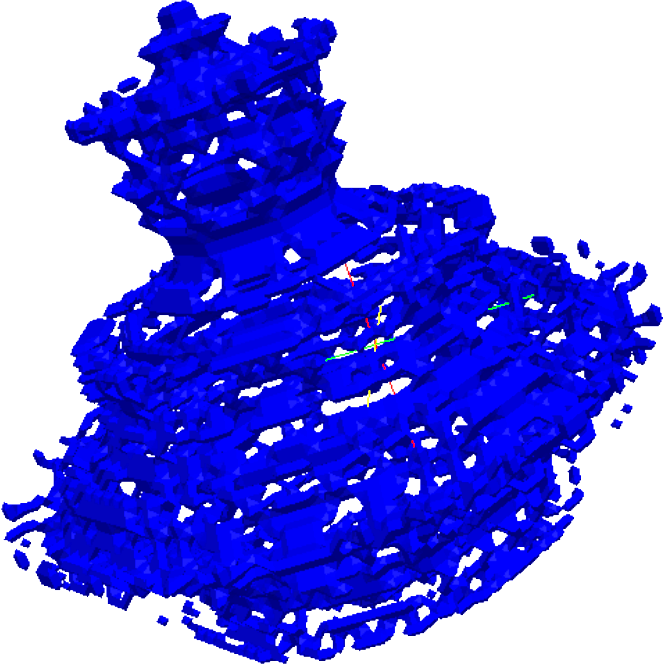
\includegraphics[width=0.5\textwidth]{apfel/pic/v1_100.png}
	\caption{3D Darstellung einer $100\times100\times 100$ Matrix}
	\label{fig. mandelbrot100}
\end{figure}
\begin{figure}[ht!]\centering
	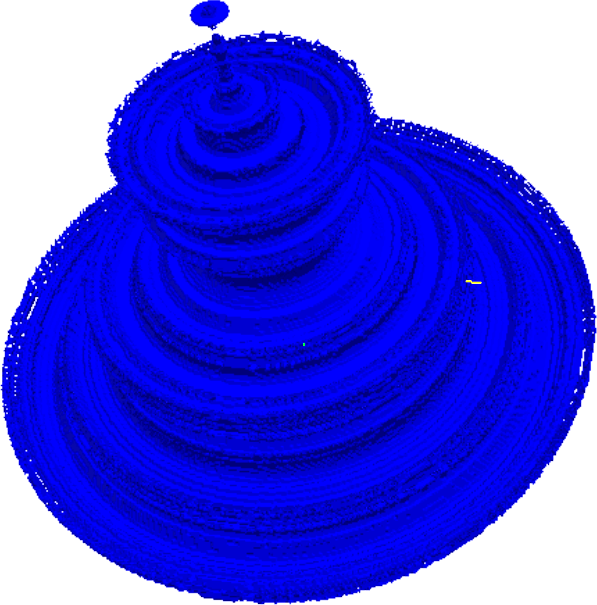
\includegraphics[width=0.5\textwidth]{apfel/pic/v2_500.png}
	\caption{3D Darstellung einer $500\times500\times 500$ Matrix}
	\label{fig. mandelbrot500}
\end{figure}
\begin{figure}[ht!]\centering
	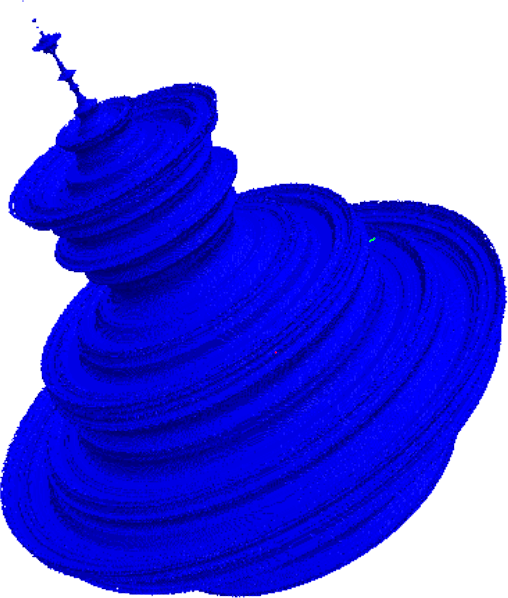
\includegraphics[width=0.5\textwidth]{apfel/pic/v2_1000.png}
	\caption{3D Darstellung einer $1000\times1000\times 1000$ Matrix}
	\label{fig. mandelbrot1000}
\end{figure}

\subsection{Komprimierung der Ausgabedaten}
Aufgrund der grossen Datenmengen lohnt sich ein kurzer Blick auf die
generierten Daten. Diese liegen im nicht komprimierten NetCDF-Format vor
und beinhalten grosse Mengen an Rohdaten, welche sich teilweise sehr
"ahnlich sind. Wird der Datentyp {\tt short} benutzt, laufen viele
Resultate "uber die speicherbare Grenze hinaus. Deshalb werden diese
manuell auf den maximal m"oglichen Wert begrenzt. Dies ergibt eine
Vielzahl an Datenwerten, welche eigentlich identisch sind. Noch extremer
wird dies, wenn das Resultat der Berechnung nur noch mit den Werten 0
(divergent) oder 1 (beschr"ankt) festgehalten wird. Die Entscheidung,
ob der Wert beschr"ankt bleibt oder nicht wird anhand eines geeigneten
Schwellwertes entschieden. Die ganze Datei enth"alt in diesem Falle nur
noch zwei verschiedene Werte. Solche Datens"atze eignen sich hervorragend
f"ur eine Komprimierung.

Als Komprimierungsverfahren wurde {\tt bzip2} verwendet. Dieses
kann sowohl normal als auch parallelisiert ({\tt pbzip2}) angewendet
werden. Die Versuche wurden ebenfalls auf dem f"ur die Berechnungen
verwendeten Cluster durchgef"uhrt. Es zeigen sich erstaunliche Resultate
(siehe Tabelle \ref{kompression}).

Sowohl bei der Verwendung von {\tt bzip2} als auch {\tt pbzip2} sinkt
die Datengr"osse drastisch. Da bei {\tt pbzip2} die Daten in parallel
komprimierbare Bl"ocke unterteilt werden, ist die Komprimierung wesentlich
weniger effizient. Die Ausf"uhrungszeit sinkt jedoch drastisch.

Es zeigt sich, dass eine Komprimierung der Daten je nach Inhalt sehr
grosse Vorteile bringen kann. Diese liegen nicht nur im ben"otigten
Speicherplatz, sondern auch bei der "Ubertragung auf ein anderes
System. So k"onnen trotz der ben"otigten Zeit zur Komprimierung und
Entpackung unter Umst"anden markante Zeitersparnisse erzielt werden. Dies
f"allt beispielsweise bei der Verwendung eines langsamen VPN-Zugangs
ins Gewicht.
\begin{table}[ht]\centering
	\begin{tabular}{|l|l|l|}
		\hline
		Verfahren & Dauer & Datengr"osse \\ \hline
		keines & 0s & 2000000116 Bytes = 1.863 GiB \\ \hline
		{\tt pbzip2} & 3s & 1615000 Bytes = 1.54 MiB \\ \hline
		{\tt bzip2} & 52s & 415734 Bytes = 405.99 KiB \\ \hline
	\end{tabular}
	\caption{Datenkompression}
	\label{kompression}
\end{table}

\printbibliography[heading=subbibliography]
\end{refsection}
